\documentclass[10pt]{article}

\usepackage[margin=0.92in]{geometry}
\usepackage[T1]{fontenc}
\usepackage{lmodern}
\usepackage{microtype}
\usepackage{setspace}
\usepackage{amsmath,amssymb,amsthm,mathtools}
\usepackage{booktabs}
\usepackage{graphicx}
\usepackage{caption}
\usepackage{subcaption}
\usepackage{algorithm}
\usepackage[noend]{algpseudocode}
\usepackage{enumitem}
\usepackage{xcolor}
\usepackage{natbib}
\usepackage{hyperref}
\usepackage[nameinlink,noabbrev]{cleveref}

\definecolor{linkblue}{RGB}{38,84,124}
\hypersetup{
  colorlinks=true,
  linkcolor=linkblue,
  citecolor=linkblue,
  urlcolor=linkblue,
  pdftitle={Geodesic Momentum Sampling for Masked Discrete Diffusion Language Models},
  pdfauthor={Yoonseong Jeong}
}

\graphicspath{{figures/}}
\setlist{nosep,leftmargin=1.5em}
\captionsetup{font=small,labelfont=bf}
\setstretch{1.075}
\setlength{\parskip}{0.18em}

\newtheorem{proposition}{Proposition}
\newtheorem{corollary}{Corollary}
\newtheorem{remark}{Remark}
\newtheorem{assumption}{Assumption}

\newcommand{\simplex}{\Delta^{V-1}}
\newcommand{\sphere}{\mathbb{S}^{V-1}}
\newcommand{\sphereplus}{\mathbb{S}^{V-1}_{+}}
\newcommand{\FR}{\mathrm{FR}}
\newcommand{\Exp}{\operatorname{Exp}}
\newcommand{\Log}{\operatorname{Log}}
\newcommand{\Slerp}{\operatorname{Slerp}}
\newcommand{\Projplus}{\operatorname{Proj}_{+}}
\newcommand{\Cat}{\operatorname{Cat}}
\newcommand{\mask}{\mathtt{m}}
\newcommand{\eps}{\varepsilon}

\title{\textbf{Geodesic Momentum Sampling for Masked Discrete Diffusion Language Models}\\
\large An Inference-Time Fisher--Rao Extrapolation Method}
\author{Yoonseong Jeong\\School of Computing, KAIST}
\date{Draft --- July 2026}

\begin{document}
\maketitle

\begin{abstract}
Masked discrete diffusion language models generate text through a sequence of categorical denoising
transitions.  We study an inference-time modification that treats each per-token categorical prediction
as a point on the Fisher--Rao statistical manifold.  The square-root map embeds the categorical simplex
into the positive orthant of a hypersphere, where closed-form spherical interpolation is available.  At
each reverse step, we recursively continue the great-circle arc from the previous extrapolated prediction
through the current model prediction, map the result back to a categorical distribution, and insert it
into the original MDLM or SEDD transition.  We call the method \emph{geodesic momentum sampling}.

We give a precise geometric derivation, prove equivalence between the unprojected update and an
exponential-map continuation, and show that its small-angle coefficients coincide with the coefficients
of variable-step Adams--Bashforth two-step extrapolation.  We also delimit this analogy: the method
extrapolates prediction distributions rather than tangent vector fields, retains stochastic categorical
jumps, and uses a positive-orthant projection.  It is therefore not a second-order probability-flow ODE
solver, and no second-order convergence claim is made.  Archived experiments on OpenWebText
checkpoints suggest improved GPT-2 generative perplexity for MDLM at 10--100 reverse steps and for SEDD
at 10--50 steps.
\end{abstract}

\section{Introduction}

Discrete diffusion language models offer parallel, bidirectional generation, but accurate sampling often
requires many reverse transitions.  MDLM \citep{sahoo2024mdlm} simplifies absorbing-state diffusion
through a substitution parameterization and provides an efficient cached sampler.  SEDD
\citep{lou2024sedd} instead learns concrete score ratios and admits an analytic reverse transition.
Both models nevertheless operate by repeatedly producing categorical distributions over a vocabulary.

Information geometry supplies a natural geometry for these distributions.  The interior of the
categorical simplex carries the Fisher--Rao metric \citep{amari2016information}; the square-root map
identifies it, up to a constant scale, with the positive orthant of a sphere.  This construction underlies
Fisher-Flow \citep{davis2024fisherflow} and the continuous Riemannian diffusion language model (RDLM)
\citep{jo2025rdlm}.  Those methods learn or simulate continuous flows on the sphere.  Our setting is
different: we preserve pretrained discrete MDLM and SEDD models and modify only their inference-time
categorical predictions.

The main contributions are:
\begin{itemize}
  \item We formulate recursive geodesic extrapolation of categorical predictions using the exact
  square-root embedding and spherical linear interpolation (SLERP).
  \item We show that the unprojected update is an exponential-map continuation and derive its local
  Adams--Bashforth-like coefficient structure.
  \item We instantiate the same geometric operator at two different interfaces: the clean-token
  prediction in MDLM and the analytic transition distribution in SEDD.
  \item We state invariants and the precise limits of the high-order analogy.
  In particular, we do not identify the algorithm with an RDLM probability-flow ODE solver.
  \item We report MDLM and SEDD quality results across six reverse-step counts.
\end{itemize}

\section{Background}

\subsection{Categorical Fisher--Rao geometry}

Let
\begin{equation}
  \simplex
  = \left\{p\in\mathbb{R}^{V}: p_k\ge 0,\ \sum_{k=1}^{V}p_k=1\right\}
\end{equation}
be the categorical probability simplex.  On its interior, a tangent vector satisfies
$\sum_k v_k=0$, and the Fisher--Rao metric is
\begin{equation}
  g_p(v,w)=\sum_{k=1}^{V}\frac{v_kw_k}{p_k}.
  \label{eq:fisher_metric}
\end{equation}

\begin{proposition}[Square-root isometry]
Define $\Psi:\operatorname{int}(\simplex)\rightarrow\sphereplus(2)$ by
$\Psi(p)=2\sqrt{p}$ elementwise, where $\sphereplus(2)$ is the positive orthant of the sphere of
radius two.  Then $\Psi$ is an isometry between the Fisher--Rao metric and the metric induced by the
ambient Euclidean space.
\end{proposition}

\begin{proof}
For $\psi_k=2\sqrt{p_k}$, we have $d\psi_k=dp_k/\sqrt{p_k}$.  Therefore
\begin{equation}
  \lVert d\psi\rVert_2^2
  =\sum_k\frac{dp_k^2}{p_k}
  =ds_{\FR}^2.
\end{equation}
Moreover, $\lVert\psi\rVert_2^2=4\sum_k p_k=4$, so $\psi$ lies on the radius-two sphere.
\end{proof}

The implementation uses the unit-sphere coordinate
\begin{equation}
  u(p)=\sqrt{p}\in\sphereplus,
  \label{eq:sqrt_map}
\end{equation}
which differs only by the constant factor two.  For $p,q\in\operatorname{int}(\simplex)$, their spherical angle is
\begin{equation}
  \omega(p,q)
  =\arccos\langle u(p),u(q)\rangle
  =\arccos\left(\sum_k\sqrt{p_kq_k}\right),
  \label{eq:bhattacharyya_angle}
\end{equation}
and the Fisher--Rao distance under the radius-two convention is $d_{\FR}(p,q)=2\omega(p,q)$.
This formula extends continuously to the closed simplex and yields its metric completion; boundary
points themselves are not smooth points of the Fisher--Rao Riemannian manifold.

\subsection{Masked discrete diffusion and MDLM}

Let $\mask$ denote an absorbing mask state and let $\sigma(t)$ be the integrated noise schedule.  The
probability of having moved to the mask by time $t$ is
\begin{equation}
  m(t)=1-\exp[-\sigma(t)].
\end{equation}
For a reverse step $t>s$, MDLM predicts a clean-token distribution
$p_{\theta,t}(\cdot\mid x_t)$ whose absorbing-state parameterization satisfies
$p_{\theta,t}(\mask\mid x_t)=0$ and $\sum_{k\ne\mask}p_{\theta,t}(k\mid x_t)=1$.
When $x_t=\mask$, the baseline implementation samples from the
unnormalized weights
\begin{equation}
  \widetilde q^{\mathrm{MDLM}}_{s\mid t}(k\mid x_t=\mask)=
  \begin{cases}
    [m(t)-m(s)]p_{\theta,t}(k\mid x_t), & k\neq\mask,\\
    m(s), & k=\mask.
  \end{cases}
  \label{eq:mdlm_transition}
\end{equation}
Their common normalization is immaterial for categorical sampling.  When $x_t\neq\mask$, the
absorbing reverse sampler copies the already unmasked token.  The cached sampler reuses
$p_{\theta,t}$ until the discrete state changes \citep{sahoo2024mdlm}.

\subsection{SEDD analytic transitions}

SEDD learns a concrete score ratio that approximates $p_t(y)/p_t(x)$
\citep{lou2024sedd}.  Let $r_\theta(x_t,t)$ denote the learned score vector, let
$\mathcal{S}_{\Delta\sigma}$ denote the staggered-score transform, and let
$K_{\Delta\sigma}(x_t,\cdot)$ denote the transported forward kernel.  The analytic sampler uses
\begin{equation}
  \widetilde q^{\mathrm{SEDD}}_{s\mid t}
  =\mathcal{S}_{\Delta\sigma}\!\left(r_\theta(x_t,t)\right)
   \odot K_{\Delta\sigma}(x_t,\cdot),
  \qquad
  \Delta\sigma=\sigma(t)-\sigma(s),
  \label{eq:sedd_transition}
\end{equation}
followed by categorical sampling.  Our SEDD variant applies geometry to the normalized version of
\cref{eq:sedd_transition}, not to the score vector itself.

\section{Geodesic Momentum Sampling}

\subsection{A common distribution interface}

For each batch element and sequence position, define a categorical distribution $z_i\in\simplex$ at
reverse index $i$:
\begin{equation}
  z_i =
  \begin{cases}
    p_{\theta,t_i}(\cdot\mid x_{t_i}), & \text{MDLM},\\
    \operatorname{Normalize}(\widetilde q^{\mathrm{SEDD}}_{t_{i+1}\mid t_i}), & \text{SEDD}.
  \end{cases}
  \label{eq:common_distribution}
\end{equation}
The raw spherical coordinate is $u_i=\sqrt{z_i}$.  Let $\widehat u_{i-1}$ be the previous
\emph{extrapolated} coordinate.  This recursive choice is important: the method has persistent momentum
rather than retaining only two raw predictions.

\subsection{Exact spherical continuation}

For unit vectors $a,b\in\sphere$ with angle $\omega=\arccos\langle a,b\rangle\in(0,\pi)$,
SLERP is \citep{shoemake1985slerp}
\begin{equation}
  \Slerp(a,b;\tau)
  =\frac{\sin[(1-\tau)\omega]}{\sin\omega}a
   +\frac{\sin(\tau\omega)}{\sin\omega}b.
  \label{eq:slerp}
\end{equation}
Interpolation uses $\tau\in[0,1]$.  We instead choose $\tau=1+\alpha_i$:
\begin{equation}
  e_i
  =\frac{\sin(-\alpha_i\omega_i)}{\sin\omega_i}\widehat u_{i-1}
   +\frac{\sin[(1+\alpha_i)\omega_i]}{\sin\omega_i}u_i,
  \quad
  \omega_i=\arccos\langle\widehat u_{i-1},u_i\rangle.
  \label{eq:geodesic_extrapolation}
\end{equation}

\begin{proposition}[Exponential-map representation]
For distinct, non-antipodal $a,b\in\sphere$ and $\alpha\ge 0$,
\begin{equation}
  \Slerp(a,b;1+\alpha)
  =\Exp_b\!\left[-\alpha\Log_b(a)\right].
  \label{eq:exp_equivalence}
\end{equation}
Thus \cref{eq:geodesic_extrapolation} exactly continues the great-circle arc from $a$ through $b$ by
an additional fraction $\alpha$ before the positivity operation described below.
\end{proposition}

\begin{proof}
The curve $\gamma(\tau)=\Slerp(a,b;\tau)$ is the unique shortest great-circle segment from $a$ to
$b$ for $\tau\in[0,1]$.  At $b=\gamma(1)$, $-\Log_b(a)$ is the forward continuation tangent with
norm $\omega$.  Applying $\Exp_b$ to the scaled vector $-\alpha\Log_b(a)$ advances by arc length
$\alpha\omega$, which is exactly $\gamma(1+\alpha)$.
\end{proof}

At $a=b$ (equivalently, $\omega=0$), we define $\Slerp(a,a;\tau)=a$ by continuous extension,
and the proposition remains valid.  Equations~\eqref{eq:slerp}--\eqref{eq:exp_equivalence} describe
the ideal, unclamped operator.  For numerical stability, the implementation evaluates the angle as
$\arccos(\operatorname{clamp}(\langle a,b\rangle,-1+\eps,1-\eps))$; hence the exact exponential-map
identity applies to the ideal operator, while the implemented rule is a stabilized approximation near
the endpoints.

\subsection{Positive-orthant projection and probability recovery}

Great-circle extrapolation may leave the positive orthant.  The archived implementation uses
\begin{equation}
  \Projplus(e)=\frac{[e]_+}{\lVert[e]_+\rVert_2},
  \qquad [e]_{+,k}=\max(e_k,0),
  \label{eq:retraction}
\end{equation}
and recovers
\begin{equation}
  \widehat z_{i,k}=(\widehat u_{i,k})^2,
  \qquad \widehat u_i=\Projplus(e_i).
  \label{eq:prob_recovery}
\end{equation}

\begin{proposition}[Probability validity]
Whenever $\lVert[e_i]_+\rVert_2>0$, the recovered vector $\widehat z_i$ lies in $\simplex$.
\end{proposition}

\begin{proof}
Each component is a square and is therefore nonnegative.  Since $\widehat u_i$ has unit norm,
$\sum_k\widehat z_{i,k}=\sum_k\widehat u_{i,k}^2=1$.
\end{proof}

This projection is a practical domain correction, not part of the exact Fisher--Rao geodesic.  It is
nonsmooth where components cross zero (and undefined when $[e]_+=0$), preventing direct inheritance
of a high-order geodesic-integrator guarantee.

\subsection{Step coefficient and the AB2 analogy}

Let the descending reverse grid be $t_0>t_1>\cdots>t_N$ and define positive step magnitudes
$h_i=t_i-t_{i+1}$.  The implementation uses
\begin{equation}
  \alpha_i=c_i\frac{h_i}{2h_{i-1}},\qquad \alpha_0=0.
  \label{eq:alpha}
\end{equation}
For SEDD, the archived runs use $c_i=1$.  For MDLM,
\begin{equation}
  c_i=c\min\left(1,\frac{h_i}{h_{\mathrm{ref}}}\right),
  \qquad c=1,\quad h_{\mathrm{ref}}=\frac{1}{50}.
  \label{eq:dynamic_damping}
\end{equation}

\begin{proposition}[Local linear form]
For fixed $\alpha$ and $\omega=\arccos\langle a,b\rangle\rightarrow0$,
\begin{equation}
  \Slerp(a,b;1+\alpha)
  =(1+\alpha)b-\alpha a+O(\omega^2).
  \label{eq:local_linear}
\end{equation}
With $c_i=1$ and $r_i=h_i/h_{i-1}$, the leading coefficients are
$(1+r_i/2,-r_i/2)$, matching the coefficients of variable-step AB2.
\end{proposition}

\begin{proof}
Using $\sin(\beta\omega)/\sin\omega=\beta+O(\omega^2)$ in
\cref{eq:slerp} with $\tau=1+\alpha$ gives
$\sin(-\alpha\omega)/\sin\omega=-\alpha+O(\omega^2)$ and
$\sin[(1+\alpha)\omega]/\sin\omega=1+\alpha+O(\omega^2)$.
\end{proof}

\begin{remark}[Why this is not Riemannian AB2]
Riemannian AB2 combines vector fields $V_i\in T_{X_i}\mathcal{M}$ after parallel-transporting
$V_{i-1}$ into $T_{X_i}\mathcal{M}$, then updates the state with an exponential map
\citep{hairer2006geometric}.  Equation~\eqref{eq:local_linear} combines \emph{points representing
categorical predictions}; it neither evaluates nor transports tangent vector fields.  Coefficient
agreement is therefore a local analogy, not an order proof.
\end{remark}

\subsection{Instantiation for MDLM and SEDD}

For MDLM, $\widehat z_i$ replaces $p_{\theta,t_i}$ in \cref{eq:mdlm_transition}; already unmasked
tokens remain fixed.  For SEDD, $\widehat z_i$ directly replaces the normalized analytic transition in
\cref{eq:sedd_transition}.  In both cases, the next token state is sampled with Gumbel-max.  The
algorithm therefore keeps all neural-network inputs discrete.

\begin{algorithm}[t]
\caption{Geodesic momentum sampling for MDLM or SEDD}
\label{alg:gms}
\begin{algorithmic}[1]
\Require pretrained model, reverse grid $t_0>\cdots>t_N$, mode $\in\{\mathrm{MDLM},\mathrm{SEDD}\}$
\State $x\gets$ all-mask prior; $\widehat u_{-1}\gets\varnothing$
\For{$i=0,\ldots,N-1$}
  \If{mode is MDLM}
    \State $z_i\gets p_{\theta,t_i}(\cdot\mid x)$
  \Else
    \State form $\widetilde q_i$ by \cref{eq:sedd_transition}; $z_i\gets\operatorname{Normalize}(\widetilde q_i)$
  \EndIf
  \State $u_i\gets\sqrt{z_i}$; compute $\alpha_i$ by \cref{eq:alpha}
  \If{$i=0$}
    \State $\widehat u_i\gets u_i$
  \Else
    \State $e_i\gets\Slerp(\widehat u_{i-1},u_i;1+\alpha_i)$
    \State $\widehat u_i\gets\Projplus(e_i)$
  \EndIf
  \State $\widehat z_i\gets\widehat u_i^{\odot2}$
  \If{mode is MDLM}
    \State insert $\widehat z_i$ into \cref{eq:mdlm_transition}; sample masked positions and copy others
  \Else
    \State $x\sim\Cat(\widehat z_i)$
  \EndIf
\EndFor
\State apply the baseline final denoising step and return $x$
\end{algorithmic}
\end{algorithm}

\section{Theoretical Scope and Non-Claims}

The method preserves several exact properties:
\begin{enumerate}
  \item \textbf{Discrete-state compatibility.} The model always receives integer token indices.
  \item \textbf{First-step equivalence.} Since $\alpha_0=0$, the first categorical transition equals
  the corresponding baseline transition under the same random draw.
  \item \textbf{Simplex validity.} Subject to the nonzero projection condition, every extrapolated
  distribution is nonnegative and normalized.
  \item \textbf{MDLM absorbing structure.} Tokens already unmasked remain fixed, exactly as in the
  uncached MDLM reverse transition.
\end{enumerate}

However, the sampled sequence $x_{t_i}$ changes stochastically, so the sequence $z_i$ is a collection
of conditional predictions along a random path, not a deterministic marginal curve $p_t$.  In SEDD,
$z_i$ is a one-step transition distribution rather than a state of a probability-flow ODE.  Moreover,
the Fisher--Rao metric is singular on the boundary $p_k=0$, while MDLM intentionally sets the mask
probability to zero and produces delta distributions for already unmasked tokens.  The square-root
representation remains numerically usable there, but smooth-manifold Taylor assumptions do not.

RDLM constructs a continuous bridge-mixture SDE on the hypersphere and trains a model conditioned on
continuous states \citep{jo2025rdlm}; Fisher-Flow learns a continuous vector field transporting
probability mass along spherical geodesics \citep{davis2024fisherflow}.  Our method does neither.
Likewise, DPM-Solver obtains high order by exploiting an exact semilinear integral form of a diffusion
ODE \citep{lu2022dpmsolver}, a structure absent from the present discrete sampler.  We therefore make
no claim of marginal preservation, local truncation error $O(h^3)$, or global convergence $O(h^2)$.

\section{Experimental Evaluation}

\subsection{Protocol}

The scripts compare MDLM against its \texttt{ddpm\_cache} sampler and SEDD against its analytic sampler.
Both use OpenWebText checkpoints in the MDLM codebase and sequence length 1024.  The reverse-step counts
are 10, 20, 50, 100, 256, and 512.  The quality metrics are:
\begin{itemize}
  \item token-weighted perplexity under GPT-2, where lower is better; and
  \item Jensen--Shannon divergence between generated and reference unigram token histograms, where
  lower is better.  References are nonempty strings from the WikiText-2 raw validation subset.
\end{itemize}

\subsection{Quality results}

\begin{table}[t]
\centering
\small
\caption{Quality results.  $\mathrm{Gain}_{\mathrm{PPL}}
=100(\mathrm{baseline}-\mathrm{geodesic})/\mathrm{baseline}$, so positive values favor geodesic
momentum.  Bold indicates the lower value within each pair.}
\label{tab:quality}
\begin{tabular}{llrrrrr}
\toprule
Model & Steps & Baseline PPL & Geodesic PPL & $\mathrm{Gain}_{\mathrm{PPL}}$ & Baseline JS & Geodesic JS \\
\midrule
MDLM & 10  & 551.953 & \textbf{407.473} & $+26.18\%$ & \textbf{0.38659} & 0.38850 \\
     & 20  & 261.453 & \textbf{212.993} & $+18.53\%$ & \textbf{0.37718} & 0.38073 \\
     & 50  & 140.075 & \textbf{120.542} & $+13.95\%$ & \textbf{0.36864} & 0.37629 \\
     & 100 & 92.421  & \textbf{81.864}  & $+11.42\%$ & 0.38260 & \textbf{0.38185} \\
     & 256 & \textbf{65.431} & 65.665 & $-0.36\%$ & \textbf{0.37828} & 0.38066 \\
     & 512 & \textbf{50.905} & 51.801 & $-1.76\%$ & 0.38224 & \textbf{0.37800} \\
\midrule
SEDD & 10  & 486.276 & \textbf{434.932} & $+10.56\%$ & \textbf{0.35628} & 0.36043 \\
     & 20  & 235.867 & \textbf{214.863} & $+8.91\%$  & 0.34810 & \textbf{0.34707} \\
     & 50  & 123.169 & \textbf{114.949} & $+6.67\%$  & 0.34771 & \textbf{0.34503} \\
     & 100 & \textbf{82.088} & 84.184 & $-2.55\%$ & 0.35678 & \textbf{0.35078} \\
     & 256 & \textbf{59.954} & 63.276 & $-5.54\%$ & \textbf{0.34519} & 0.34670 \\
     & 512 & 51.695 & \textbf{50.903} & $+1.53\%$ & \textbf{0.36408} & 0.36661 \\
\bottomrule
\end{tabular}
\end{table}

\begin{figure}[t]
  \centering
  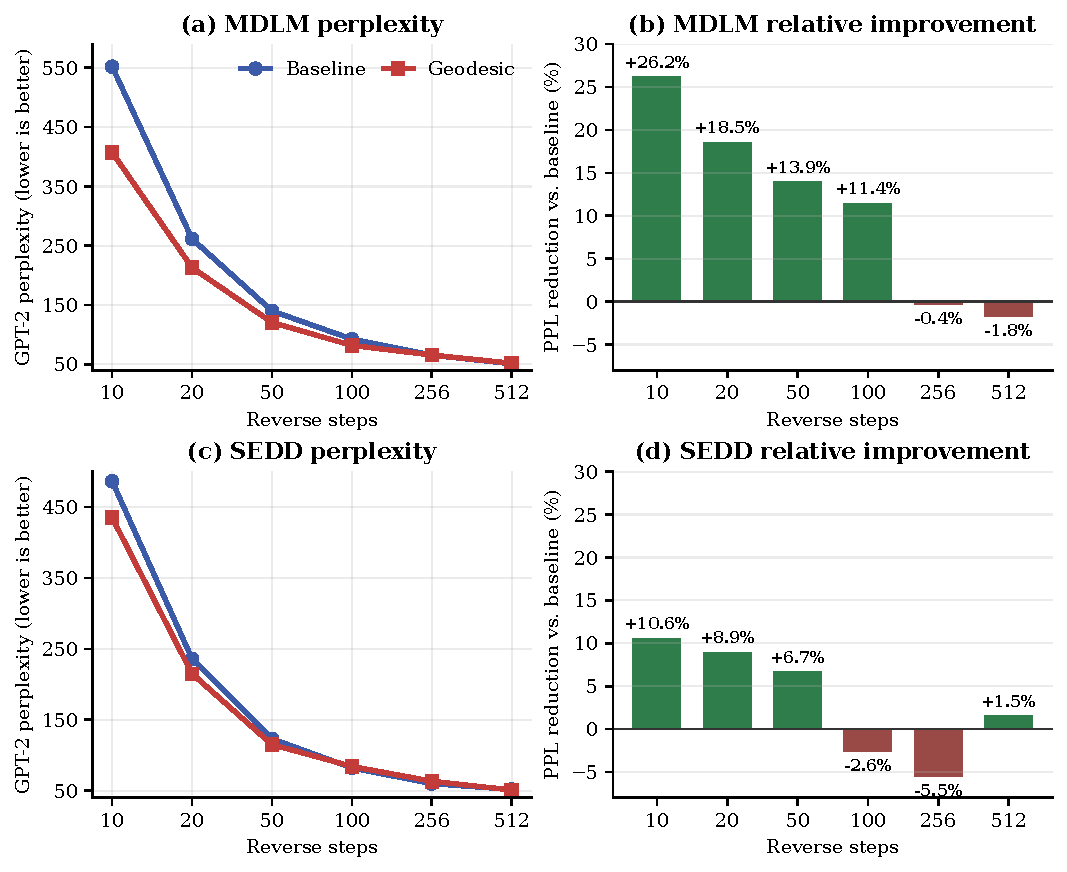
\includegraphics[width=0.94\linewidth]{quality_curves.pdf}
  \caption{Perplexity results.  Left panels show raw GPT-2 perplexity on linear vertical axes
  fitted separately to each model's observed range, making the low-step gaps directly visible.  Right panels
  show the relative PPL reduction $(\mathrm{baseline}-\mathrm{geodesic})/
  \mathrm{baseline}$, so positive bars indicate improvement and negative bars indicate degradation.
  Both improvement panels retain the same $[-8,30]$ percentage-point range.}
  \label{fig:quality_curves}
\end{figure}

At 10, 20, 50, and 100 MDLM steps, the geodesic samples have respectively 26.18\%, 18.53\%,
13.95\%, and 11.42\% lower GPT-2 perplexity.  At 256 and 512 steps, the difference vanishes and slightly
favors the baseline.  This pattern is consistent with the method's intended use as a low-step correction.
The MDLM damping in
\cref{eq:dynamic_damping} also decreases $\alpha$ beyond 50 uniform steps: approximately $0.25$ at
100, $0.098$ at 256, and $0.049$ at 512.

SEDD shows smaller perplexity reductions at 10--50 steps, degradation at 100--256, and a small
improvement at 512.  Its implementation used $\alpha=1/2$ after the first step on every uniform
grid, without MDLM's high-step damping.  This may contribute to overshoot, but the available experiment
does not isolate the cause.  Jensen--Shannon divergence is mixed for both models and does not show a
consistent distributional improvement.

\section{Discussion}

\paragraph{Interpretation.}
The strongest defensible interpretation is prediction-lag correction.  With few reverse steps, successive
denoiser or transition distributions can move substantially.  Continuing their recent Fisher--Rao arc may
anticipate the next prediction and improve quality.  As the grid is refined, raw predictions change less,
so extrapolation offers little benefit and can amplify stochastic or model error.

\paragraph{MDLM versus SEDD.}
MDLM applies momentum to a clean-token prediction before the absorbing transition and freezes completed
tokens.  SEDD applies momentum to a stochastic-state-dependent one-step transition.  The latter object may
be less temporally smooth, which weakens the curve-extrapolation interpretation and is consistent with the
less stable archived trend.

\paragraph{Relationship to continuous geometric models.}
The method uses the same Fisher--Rao embedding as Fisher-Flow and RDLM but not their dynamics.  A genuine
Riemannian multistep solver would require a continuous state $X_t$, a well-defined tangent vector field,
parallel transport between $T_{X_{i-1}}\mathcal{M}$ and $T_{X_i}\mathcal{M}$, and an exponential-map state
update.  Establishing such a solver for pretrained discrete MDLM or SEDD would require a new derivation
connecting their categorical predictions to a continuous vector field.

\section{Limitations}

\begin{enumerate}
  \item \textbf{No convergence order.} Stochastic jumps, point rather than vector extrapolation, recursive
  history, and nonsmooth projection invalidate a direct AB2 order argument.
  \item \textbf{Boundary geometry.} Exact zeros place predictions on the boundary where the Fisher--Rao
  metric is singular.
  \item \textbf{Position-wise approximation.} Each token position is treated as a separate categorical
  simplex.  The geometry of the full joint sequence distribution is not represented.
\end{enumerate}

\section{Conclusion}

We presented geodesic momentum sampling, an inference-time modification for MDLM and SEDD that
recursively extrapolates categorical predictions on the Fisher--Rao square-root sphere.  The update has an
exact exponential-map interpretation before positive-orthant projection, and its local coefficients match
variable-step AB2 coefficients.  The algorithm nevertheless operates on prediction points along a stochastic
discrete path, not on parallel-transported vector fields of a probability-flow ODE.  Its mathematically
accurate characterization is therefore \emph{recursive Fisher--Rao spherical extrapolation}, not a proven
second-order Riemannian solver.

Results show promising low-step perplexity behavior, especially for MDLM, while distributional metrics and
higher-step SEDD behavior are mixed.  A derivation based on a continuous vector field remains necessary for
formal convergence claims.

\bibliographystyle{plainnat}
\bibliography{references}

\end{document}
